\section{Auswertung}
\label{sec:Analysis}

Für die Auswertung wurden mit dem DRS Bord bei verschiedenen Bias Spannungen und Laser Intensitäten jeweils 1000 Events aufgezeichnet. 
Alle gezeigten Signalformen dieser Events wurden mit einem Gauß-Filter ($\sigma = 2$) geglättet. 
Die Messungen wurden sowohl von der Vorderseite als auch von der Rückseite durchgeführt, um jeweils die Signale der Elektronen bzw. Löcher zu untersuchen.



\subsection{Vergleich der mittleren Wellenformen}
\label{sec:waveforms}
In \autoref{fig:mean_vorder} und \autoref{fig:mean_rueck} sind die gemessenen Spannungen über Zeit dargestellt, 
in abhängigkeit von der Bias-Spannung.
Die Signale wurden jeweils mit einem Gauß-Filter geglättet und über 1000 Events gemittelt, um die dargestellte mittlere Wellenform zu erhalten.
Anhand dieser Wellenformen kann zwischen den gemessenen Signalen von Elektronen (Vorderseite) und Löchern (Rückseite) unterschieden werden, 
da die Ladungsträger ungleiche Signalformen aufweisen.
Da das elektrische Feld im Sensor nicht homogen ist werden Elektronen und Löcher untzerschiedlich zu den Elerktroden getrieben.
Die Elektronen verlieren ein Teil ihrer Geschwindigkeit,
was sich in einem abnehmenden Signal über die Zeit widerspiegelt wie in \autoref{fig:mean_vorder} zu erkennen. 
Während die Löcher beschleunigen, was zu einem ansteigende Signal führt wie in \autoref{fig:mean_rueck} zu sehen.  
\begin{figure}[htbp]
  \centering
  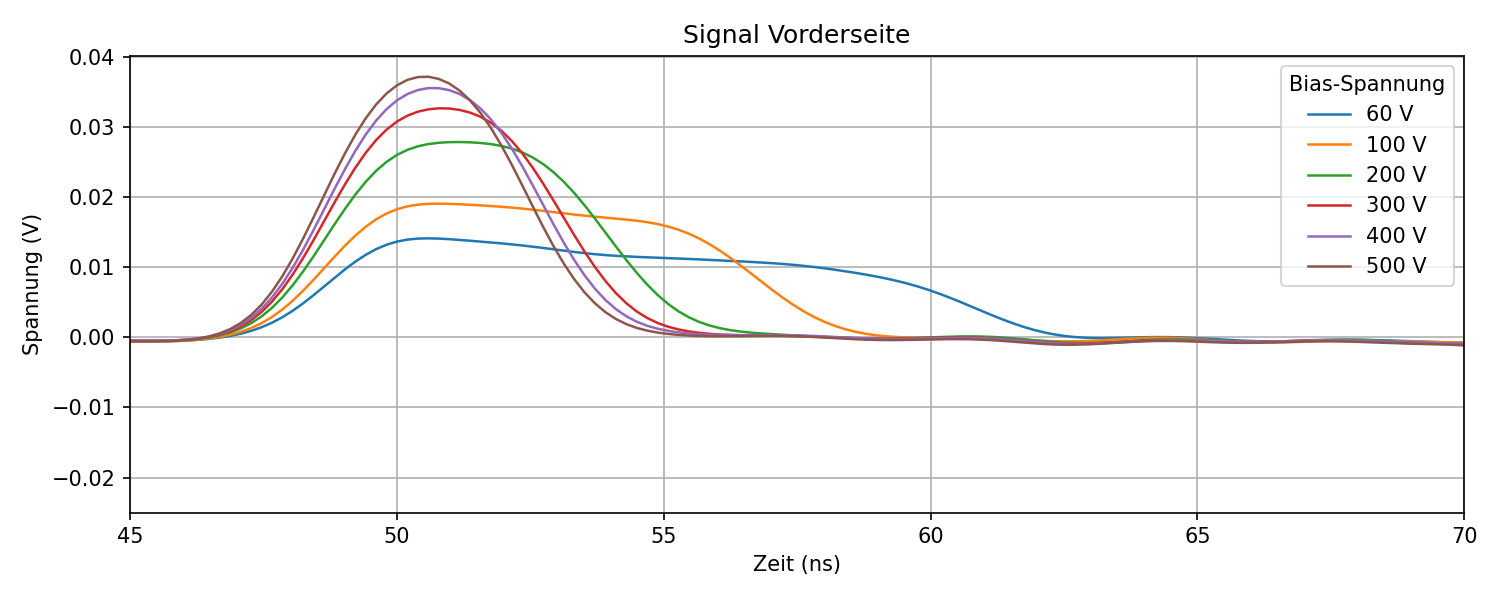
\includegraphics[width=\textwidth]{Auswertung/mean_waveforms_vorderseite.png}
    \caption{Mittlere Waveforms für verschiedene Bias-Spannungen, Vorderseite des Detektors. Das abnehmende  Signal stammt hauptsächlich von den Elektronen, die durch den Abnehmenden Feldgradienten driften.}
  \label{fig:mean_vorder}
\end{figure}
\begin{figure}[htbp]
  \centering
  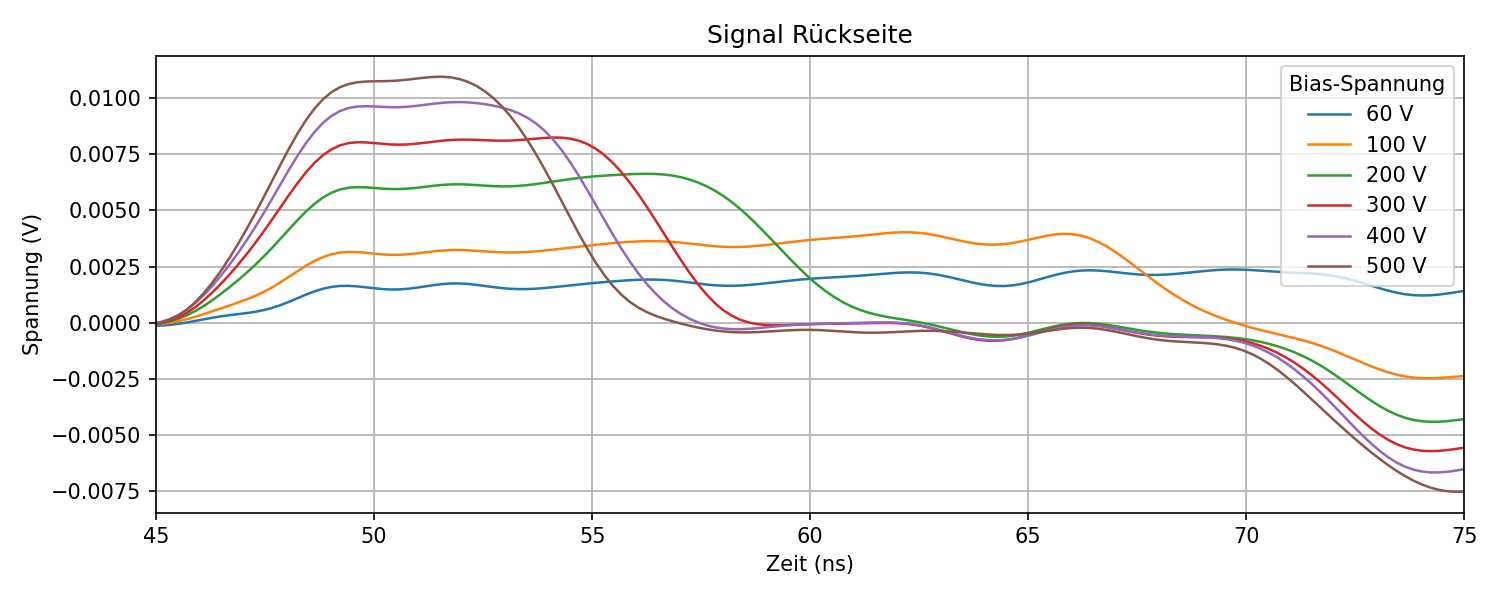
\includegraphics[width=\textwidth]{Auswertung/mean_waveforms_rueckseite.png}
  \caption{Mittlere Wellenform für verschiedene Bias-Spannungen, Rückseite des Detektors. Das steigende Signal stammt hauptsächlich von den Löchern, die durch den zunehmenden Feldgradienten beschleunigt werden.}
  \label{fig:mean_rueck}
\end{figure}
Mit steigender Bias-Spannung werden die Signale kürzer und die Amplitude größer. 
Dies ist konsistent mit einem stärkeren externen elektrischen Feld, 
das die Ladungsträger schneller zur Elektrode treibt,
was zu einem kürzerem aber größerem Signal führt. 

In \autoref{fig:mean_vorder_laser} und \autoref{fig:mean_rueck_laser} sind die mittleren Wellenformen für verschiedene Laserintensitäten dargestellt.
Diese wurden bei einem festen Bias von $V = \SI{-150}{\volt}$ aufgenommen.
Die Signale sind ebenfalls mit einem Gauß-Filter geglättet und über 1000 Events gemittelt.
Die Form der Signale bleibt dabei nahezu zeitlich konstant, 
da die Laserintensität nur die Anzahl der erzeugten Elektron-Loch-Paare beeinflusst, 
nicht aber das elektrische Feld oder die Driftgeschwindigkeit der Ladungsträger.
Je höher die Laserintensität, desto mehr Ladungsträger werden erzeugt, was zu einer größeren Amplitude der Signale führt, wie in den Abbildungen zu erkennen ist. 
\begin{figure}[htbp]
  \centering
  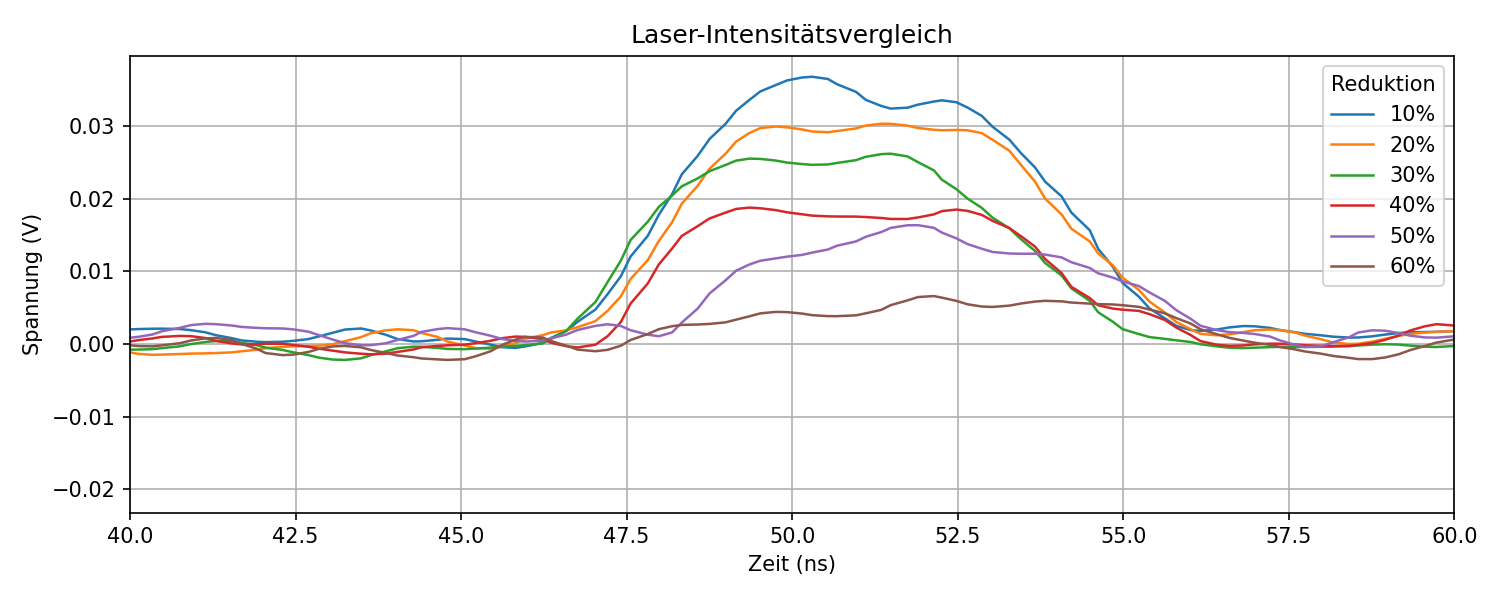
\includegraphics[width=\textwidth]{Auswertung/laser_intensitaet_vergleich.png}
    \caption{Mittlere Waveforms für verschiedene Laserintensitäten, Vorderseite des Detektors. Das höhere Signal stammt durch die erhöhte Erzeugung von Elektronen durch die erhöhte Laserintensität.}
  \label{fig:mean_vorder_laser}
\end{figure}
\begin{figure}[htbp]
  \centering
  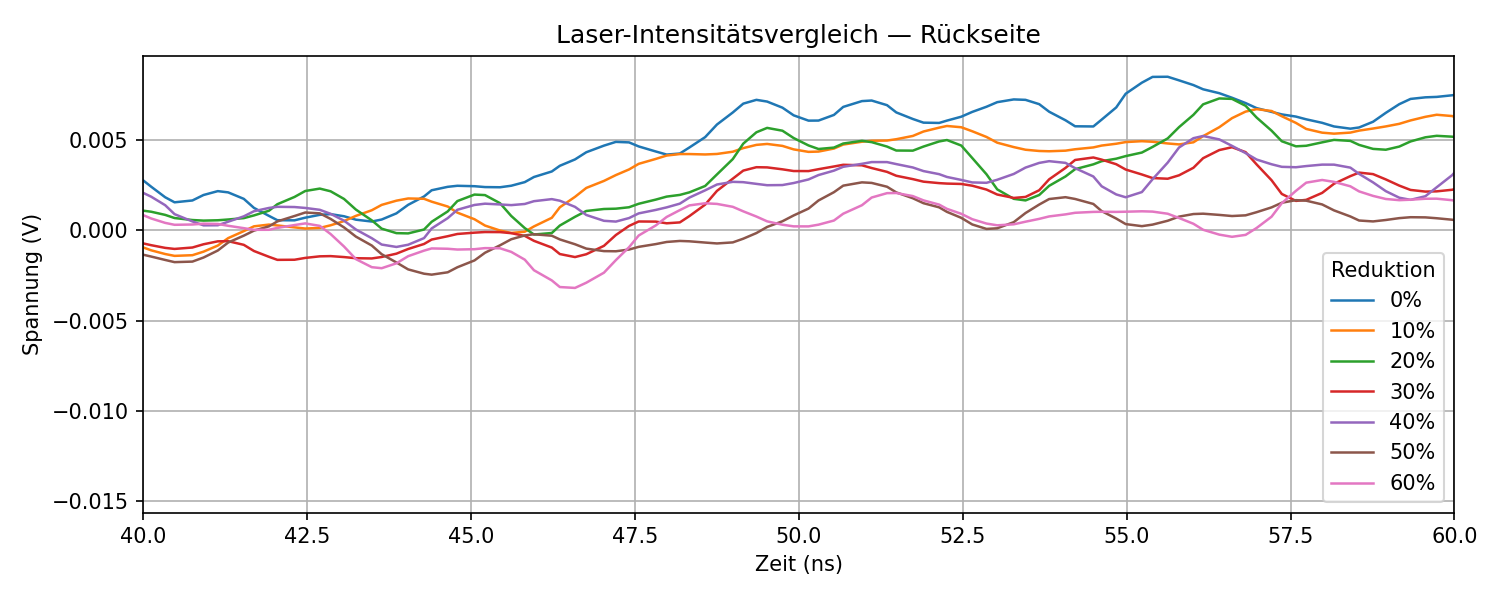
\includegraphics[width=\textwidth]{Auswertung/laser_intensitaet_vergleich_rueckseite.png}
  \caption{Mittlere Wellenform für verschiedene Laserintensitäten, Rückseite des Detektors. Das höhere Signal stammt durch die erhöhte Erzeugung von Löchern durch die erhöte Laserintensität.}
  \label{fig:mean_rueck_laser}
\end{figure}



\subsection{Ladung in Abhängigkeit von Bias-Spannung und Ladungsträgertyp}
\label{sec:charge}
Die in einem Event erzeugte Ladung $Q$ kann durch
\begin{equation}
  Q = \int i(t)\,\mathrm{d}t = \frac{1}{R}\int U(t)\,\mathrm{d}t
  \label{eqn:charge}
\end{equation}
berechnet werden, wobei $R = 50\,\Omega$ der Widerstand des Messsystems ist und $U(t)$ die Spannung über die Zeit beschreibt.
Somit lässt sich die erzeugte Ladung bestimmen, indem über das gemessene Signal integriert wird. 
\autoref{fig:charge_bias} zeigt die berechnete gemittelte Ladung als Funktion der Bias-Spannung,
sowohl für die Vorder- als auch für die Rückseite.
Für die Berechnung wurde der Peak des Signals mittels der Python-Bibliothek \texttt{scipy.signal.find\_peaks} bestimmt.
Für die Integrationsgrenzen wurden durch eine Abweichung von $5\,\%$ des Rauschpegels über und unter dem Peak gewählt.
Das Rauschen wurde durch die ersten 1000 Messpunkte eines Events bestimmt, bevor der Laser gepulst wurde.
Aufgrund des hohen Rauschens bei Bias-Spannungen von unter $100$ Volt  konnten diese Werte nicht zuverlässig bestimmt werden und wurden daher nicht in die Auswertung einbezogen.
\begin{figure}[htbp]
  \centering
  \begin{subfigure}[b]{0.49\textwidth}
    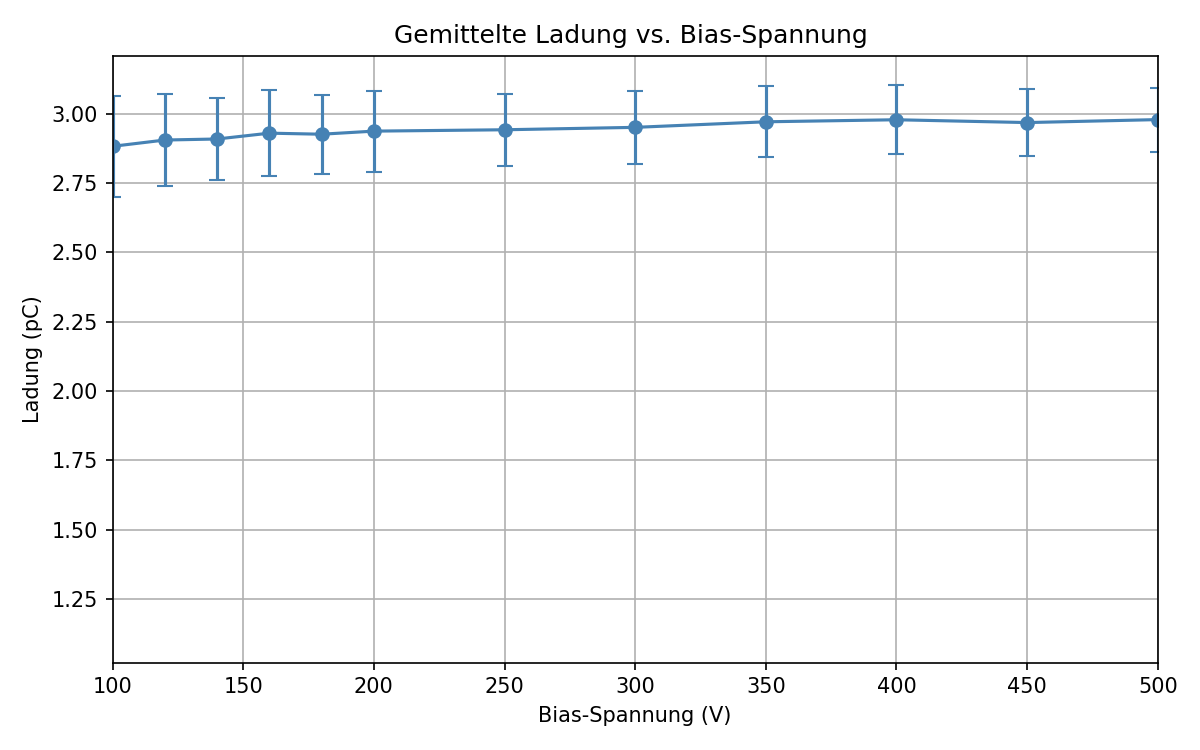
\includegraphics[width=\textwidth]{Auswertung/charge_vs_bias.png}
    \caption{Vorderseite (Elektronen)}
    \label{fig:charge_bias_v}
  \end{subfigure}
  \hfill
  \begin{subfigure}[b]{0.49\textwidth}
    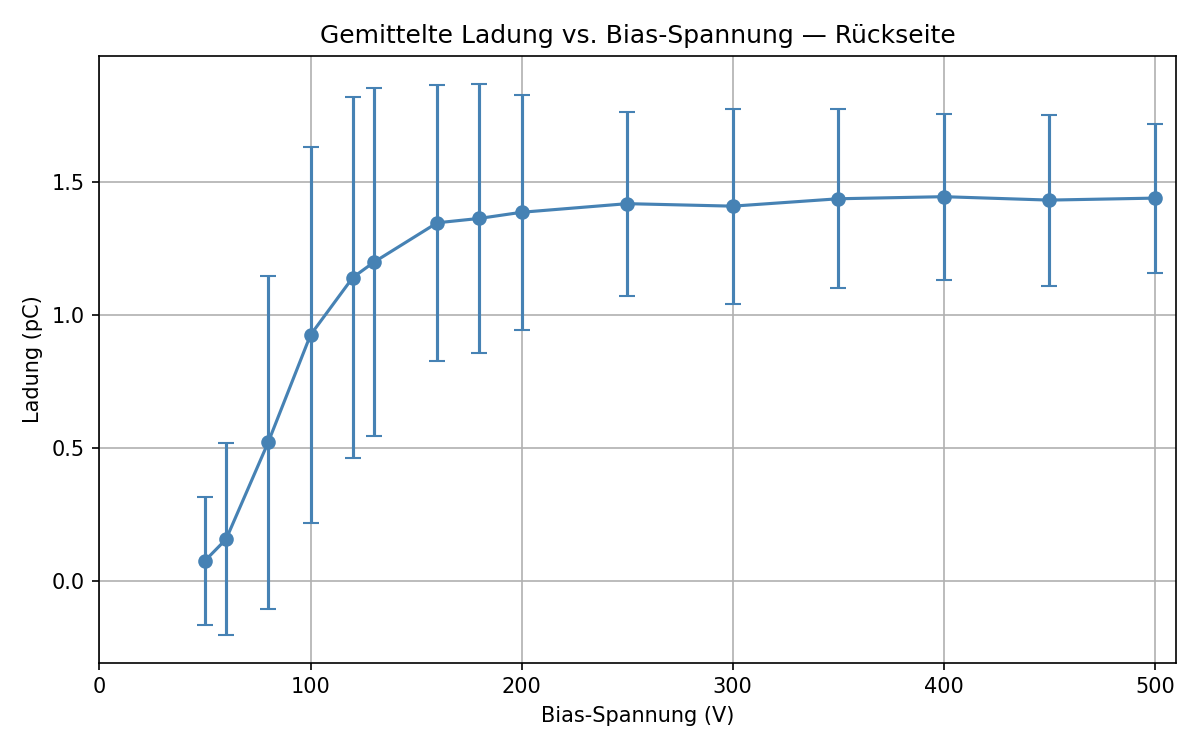
\includegraphics[width=\textwidth]{Auswertung/charge_vs_bias_rueckseite.png}
    \caption{Rückseite (Löcher)}
    \label{fig:charge_bias_r}
  \end{subfigure}
  \caption{Gemittelte induzierte Ladung als Funktion der Bias-Spannung. Fehlerbalken geben die Standardabweichung über 1000 Events an.}
  \label{fig:charge_bias}
\end{figure}
Zu beobachten ist das die gemessene Ladung unabhängig von der Bias-Spannung ist, 
da die Anzahl der erzeugten Elektron-Loch-Paare durch die Laserintensität bestimmt wird und nicht durch das elektrische Feld. 

In \autoref{fig:charge_laser} ist der berechnete Strom in Abhängigkeit der Laserintensität aufgetragen.
Durch Integration über die Siganle wurde auch hier wie oben beschrieben die Ladung bestimmt.
\begin{figure}[htbp]
  \centering
  \begin{subfigure}[b]{0.49\textwidth}
    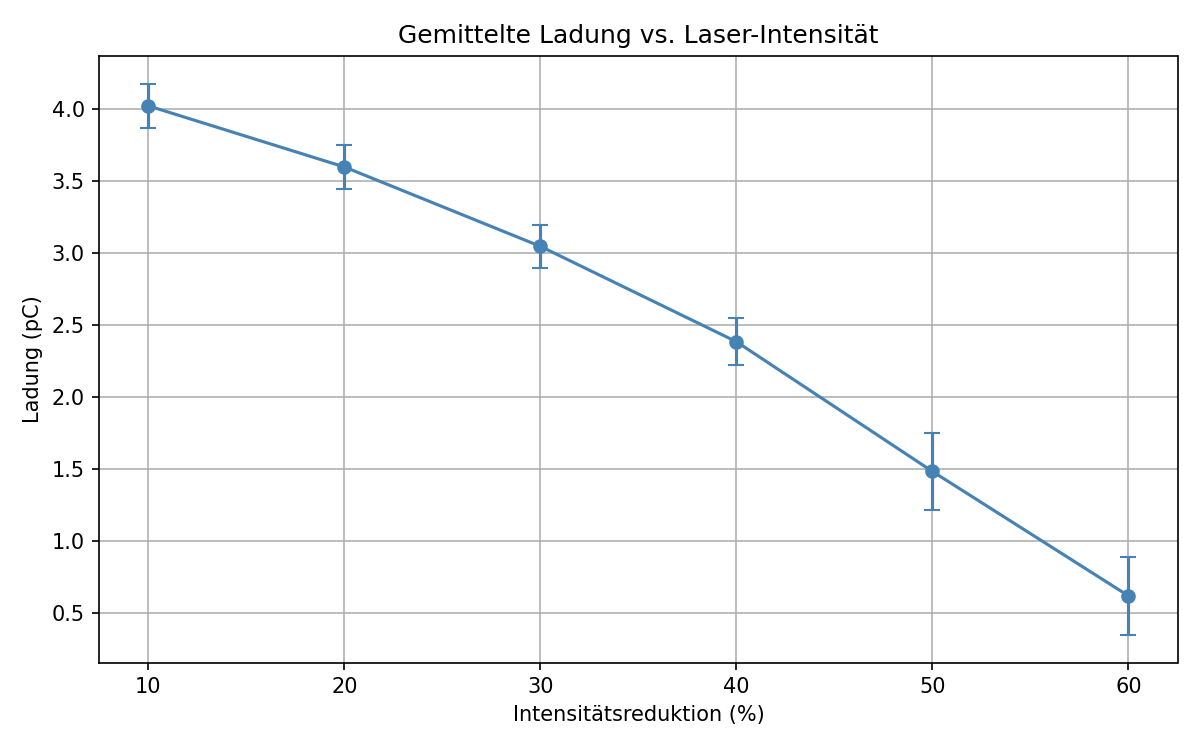
\includegraphics[width=\textwidth]{Auswertung/charge_vs_laser.png}
    \caption{Vorderseite}
    \label{fig:charge_laser_v}
  \end{subfigure}
  \hfill
  \begin{subfigure}[b]{0.49\textwidth}
    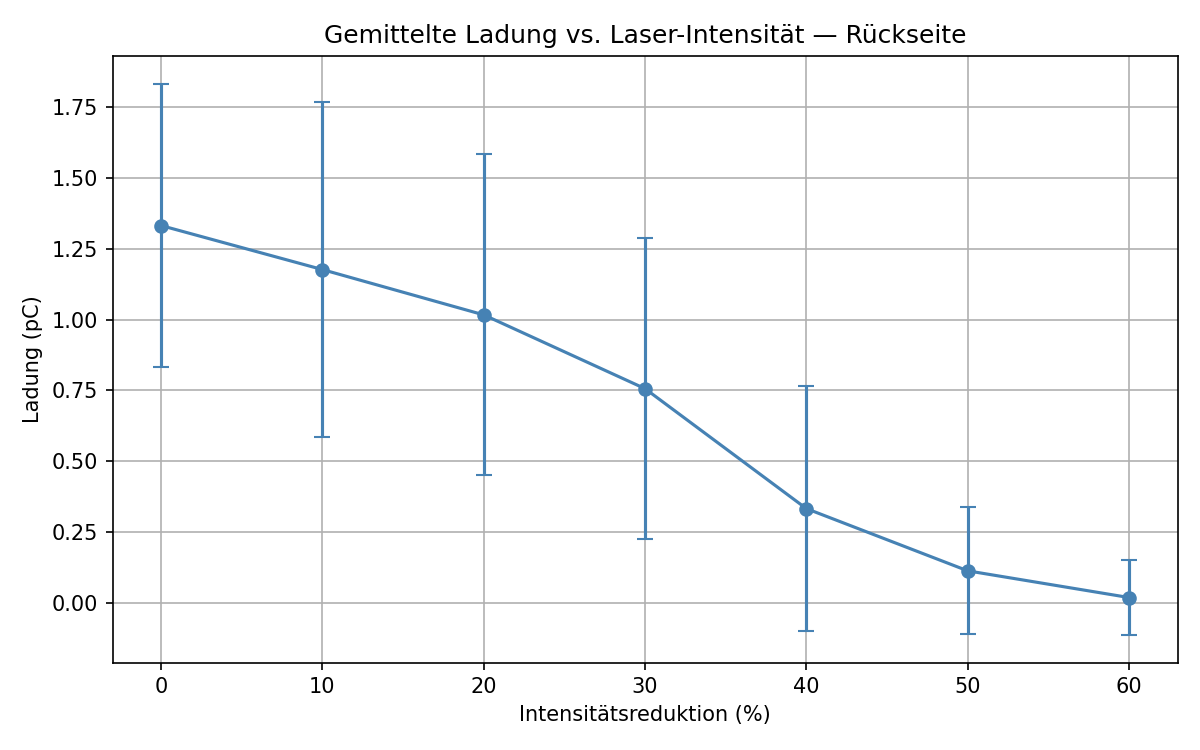
\includegraphics[width=\textwidth]{Auswertung/charge_vs_laser_rueckseite.png}
    \caption{Rückseite}
    \label{fig:charge_laser_r}
  \end{subfigure}
  \caption{Gemittelte induzierte Ladung als Funktion der Laserintensitätsreduktion. Eine Reduktion von $x\,\%$ entspricht einer Pulsbreite von $(100-x)\,\%$. Fehlerbalken geben die Standardabweichung über 1000 Events an.}
  \label{fig:charge_laser}
\end{figure}
Die Ladung sinkt mit abnehmender Laserintensität, da weniger Elektron-Loch-Paare erzeugt werden.



\subsection{Signaldauer in Abhängigkeit von Bias-Spannung und Ladungsträgertyp}
\label{sec:signaldauer}
Die Signaldauer ist definiert als die zeitliche Breite des Pulses vom Anstieg bis zum Abfall auf Rauschpegelniveau. 
\autoref{fig:sigtime_bias} zeigt die gemittelte Signaldauer als Funktion der Bias-Spannung für beide Sensororientierungen.
\begin{figure}[htbp]
  \centering
  \begin{subfigure}[b]{0.49\textwidth}
    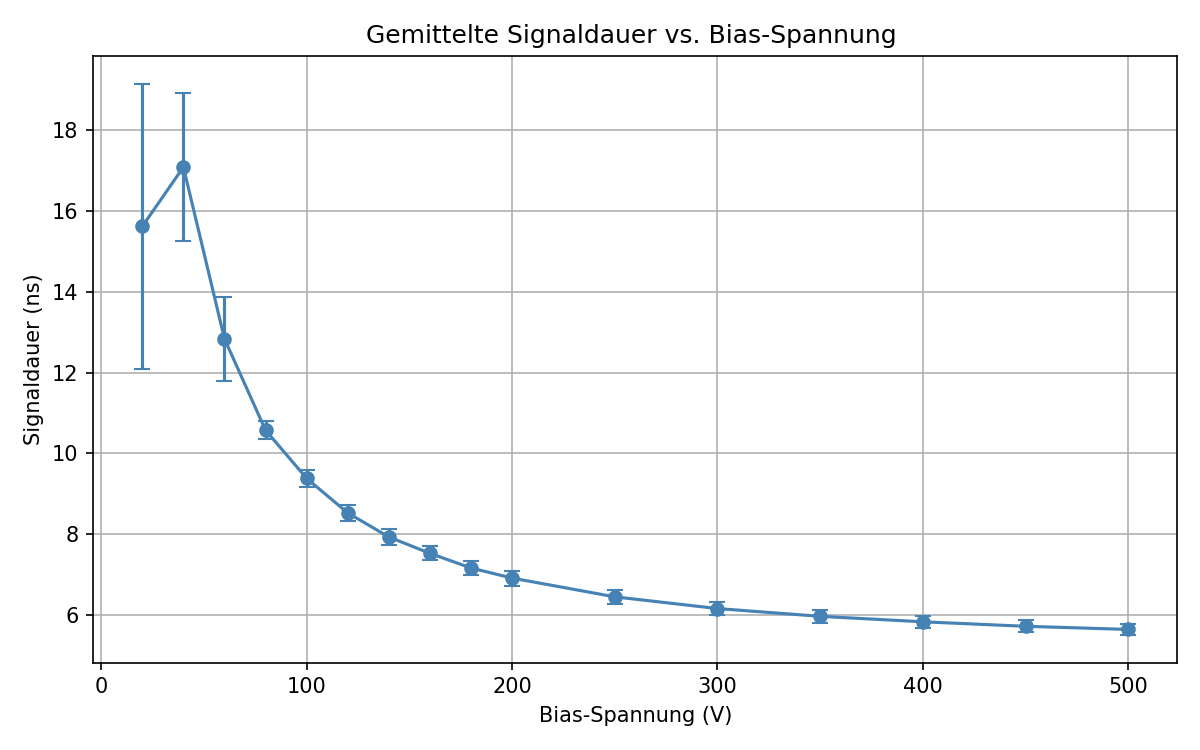
\includegraphics[width=\textwidth]{Auswertung/signalzeit_vs_bias.png}
    \caption{Vorderseite (Elektronen)}
    \label{fig:sigtime_v}
  \end{subfigure}
  \hfill
  \begin{subfigure}[b]{0.49\textwidth}
    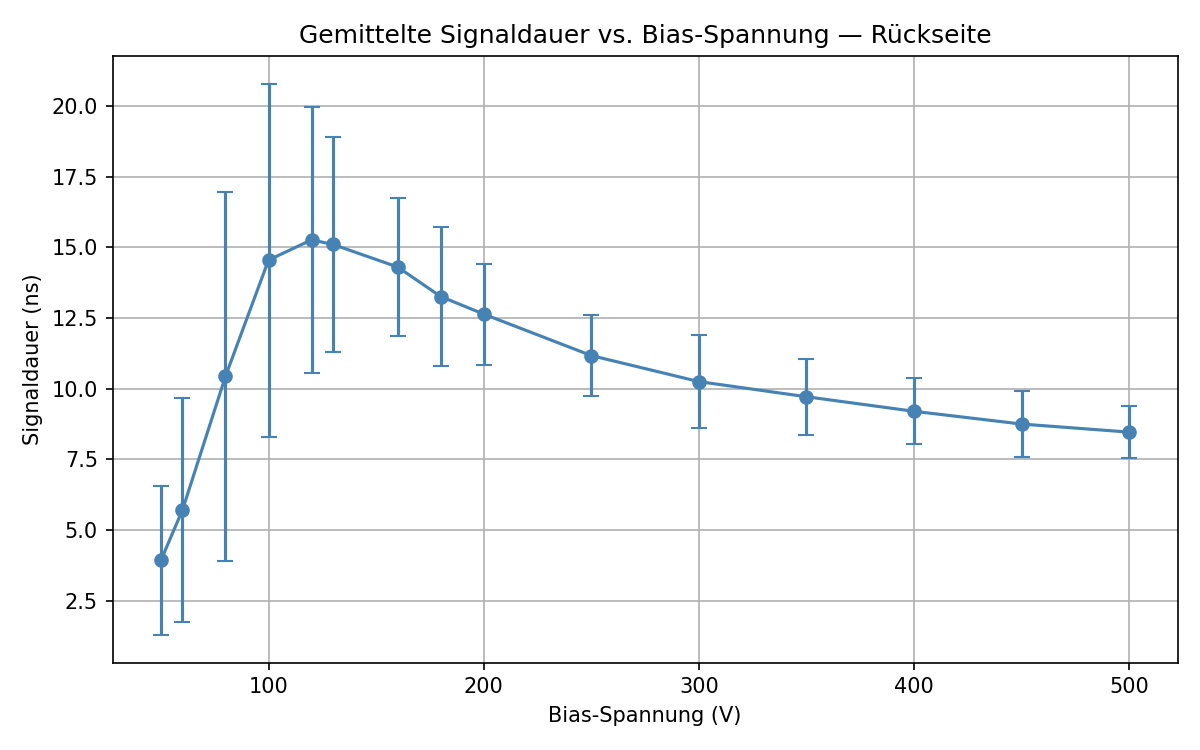
\includegraphics[width=\textwidth]{Auswertung/signalzeit_vs_bias_rueckseite.png}
    \caption{Rückseite (Löcher)}
    \label{fig:sigtime_r}
  \end{subfigure}
  \caption{Gemittelte Signaldauer als Funktion der Bias-Spannung. Mit steigender Spannung sinkt die Signaldauer, da das elektrische Feld stärker wird und die Ladungsträger schneller driften. Aufgrund des hohen Rauschens bei Bias-Spannungen von unter $100$ Volt konnten diese Werte nicht zuverlässig bestimmt werden.}
  \label{fig:sigtime_bias}
\end{figure}
Mit steigendem Bias sinkt die Signaldauer, da das elektrische Feld stärker wird und die Ladungsträger schneller zur Elektrode getrieben werden.
Die Signaldauer der Rückseite (Löcher) liegt bei gleicher Spannung durchgehend über der der Vorderseite (Elektronen). 
Dies spiegelt die geringere Mobilität der Löcher gegenüber den Elektronen wider ($\mu_h < \mu_e$).

In \autoref{fig:sigtime_laser} ist die gemittelte Signaldauer als Funktion der Laserintensität dargestellt.
\begin{figure}[htbp]
  \centering
  \begin{subfigure}[b]{0.49\textwidth}
    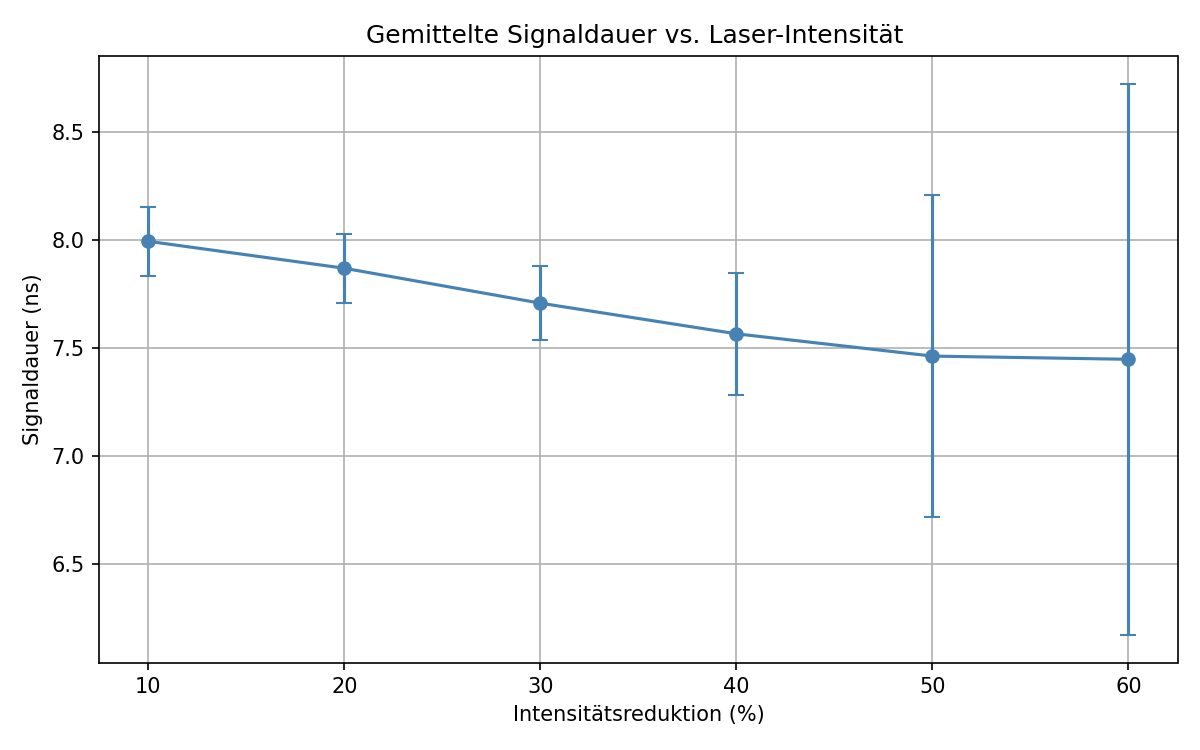
\includegraphics[width=\textwidth]{Auswertung/signalzeit_vs_laser.png}
    \caption{Vorderseite}
  \end{subfigure}
  \hfill
  \begin{subfigure}[b]{0.49\textwidth}
    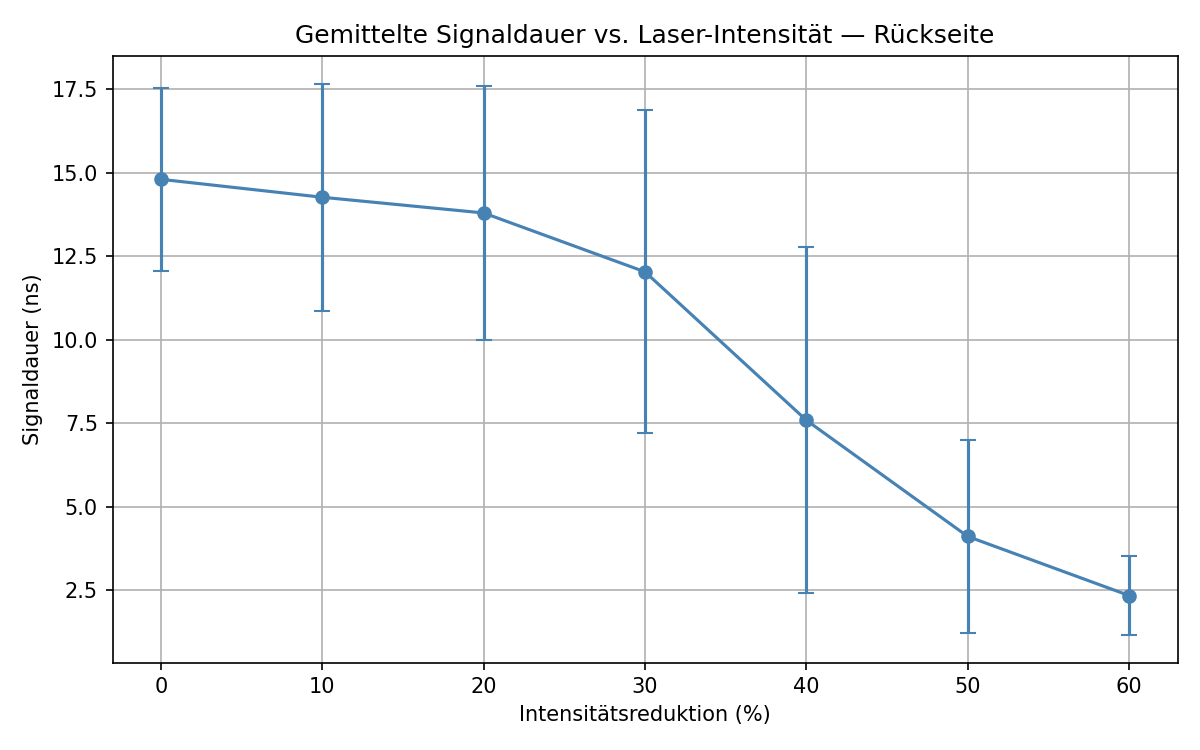
\includegraphics[width=\textwidth]{Auswertung/signalzeit_vs_laser_rueckseite.png}
    \caption{Rückseite}
  \end{subfigure}
  \caption{Gemittelte Signaldauer als Funktion der Laserintensitätsreduktion. Die Signaldauer zeigt keine signifikante Abhängigkeit von der Laserintensität.}
  \label{fig:sigtime_laser}
\end{figure}
Die Signaldauer zeigt keine signifikante Abhängigkeit von der Laserintensität, 
da diese nur die Anzahl der erzeugten Ladungsträger beeinflusst, 
nicht aber die Driftgeschwindigkeit oder das elektrische Feld, welche die Signaldauer bestimmen.



\subsection{Mobilitätsbestimmung}
\label{sec:mobilitaet}
Die Sammelzeiten $T^-$ und $T^+$ nach \autoref{eqn:T1} und \autoref{eqn:T2} vereinfachen sich für die jeweiligen Startpositionen $x_0 = 0$ (Vorderseite) und $x_0 = d$ (Rückseite) mit den Abkürzungen aus \autoref{eqn:E_neu} zu
\begin{equation}
  T^{-/+}(V) = \tau_{e/h} \cdot \ln\!\left(\frac{|V| + V_\text{dep}}{|V| - V_\text{dep}}\right)
  \qquad \text{mit} \qquad \tau_{e/h} = \frac{d^2}{2\,\mu_{e/h}\,V_\text{dep}}\,.
  \label{eqn:fit}
\end{equation}
Diese Funktion wird an die gemessene Signaldauer als Funktion von $|V|$ gefittet, wobei $\mu_{e/h}$ der einzige freie Parameter ist.


Der Fit liefert folgende Mobilitäten:
\begin{align}
  \mu_e &= \SI{1373 \pm 15}{\centi\meter\squared\per\volt\per\second}\,, \label{eqn:mu_e_result} \\
  \mu_h &= \SI{381 \pm 3}{\centi\meter\squared\per\volt\per\second}\,. \label{eqn:mu_h_result}
\end{align}
Der angegebene Fehler stammt aus der Kovarianzmatrix des Fits (\texttt{scipy.optimize.curve\_fit}) bei absoluter Fehlergewichtung durch die Standardabweichung der gemittelten Signaldauer.
In \autoref{fig:mobility_e} und \autoref{fig:mobility_h} sind die Fit-Ergebnisse für die Elektronen bzw. Löcher dargestellt.
\begin{figure}[htbp]
  \centering
  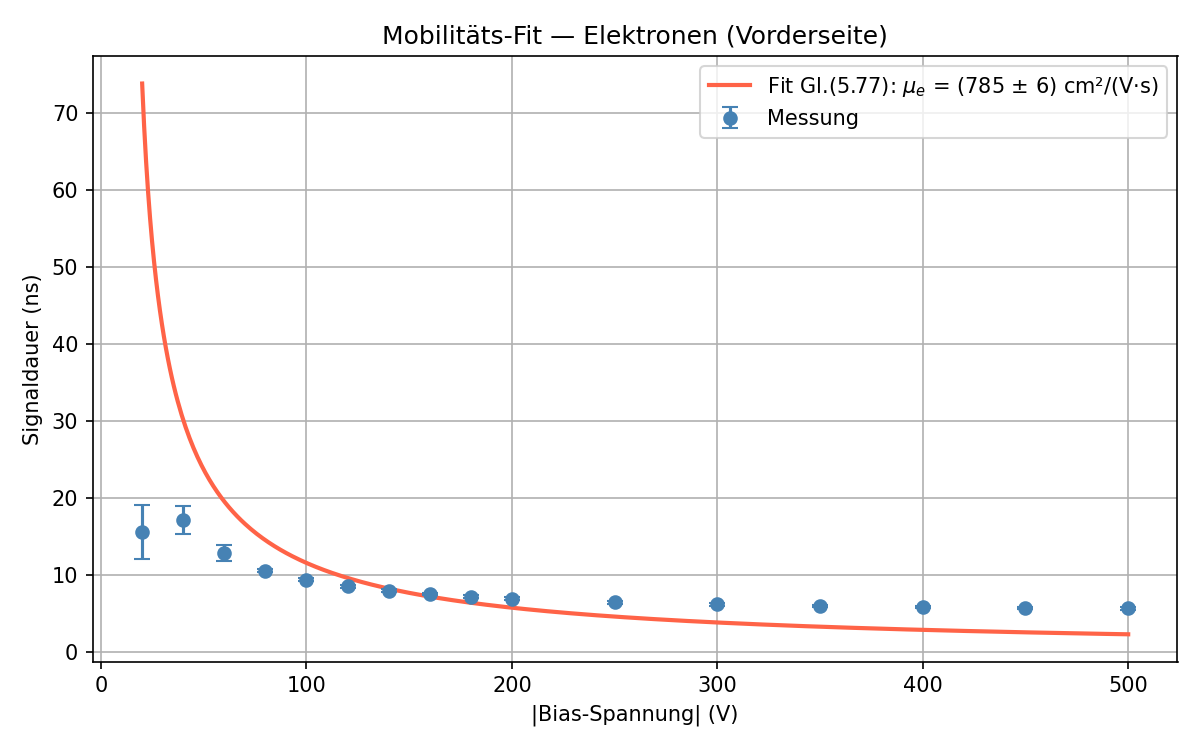
\includegraphics[width=0.8\textwidth]{Auswertung/mobilitaet_elektronen_vorderseite.png}
  \caption{Fit der Sammelzeit \autoref{eqn:fit} an die gemessene Signaldauer der Vorderseite (Elektronen).}
  \label{fig:mobility_e}
\end{figure}
\begin{figure}[htbp]
  \centering
  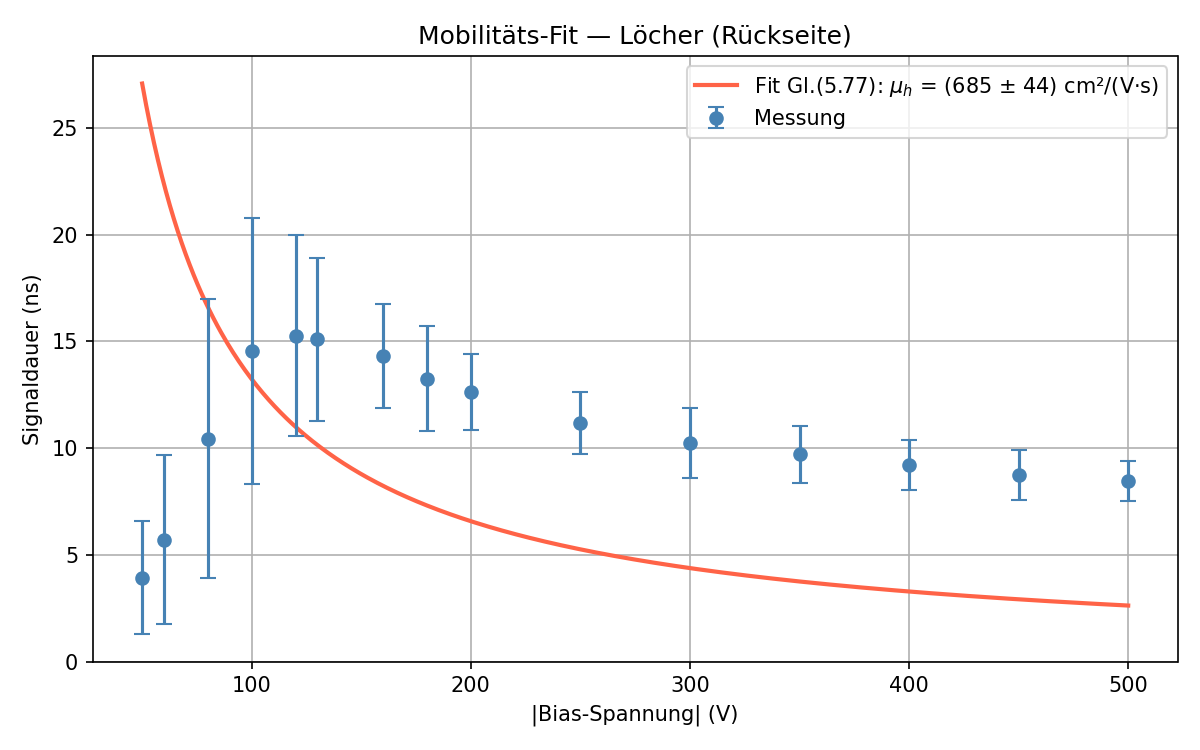
\includegraphics[width=0.8\textwidth]{Auswertung/mobilitaet_loecher_rueckseite.png}
  \caption{Fit der Sammelzeit \autoref{eqn:fit} an die gemessene Signaldauer der Rückseite (Löcher).}
  \label{fig:mobility_h}
\end{figure}
Die gemessenen Mobilitäten liegen im erwarteten Bereich für Silizium bei Raumtemperatur,
die für Elektronen $1400$ cm²/V·s und für Löcher $450$ cm²/V·s betragen \cite{Wermes}.
